\chapter{Diseño y arquitectura}\label{cap:diseno_y_arquitectura}

En este capítulo se describe la estructura técnica y conceptual sobre la que se asienta el sistema, detallando las decisiones arquitectónicas que garantizan su correcto funcionamiento, mantenibilidad y rendimiento. El diseño propuesto responde tanto a los requisitos funcionales del proyecto como a sus restricciones operativas: la ejecución de cuestionarios en tiempo real, la baja latencia en la transmisión de eventos a múltiples participantes simultáneos y una rigurosa separación de responsabilidades entre el cliente y el servidor.

\section{Patrones arquitectónicos elegidos}

Antes de seleccionar el \textit{stack} y la estructura del código, se establecieron una serie de principios de diseño orientados a garantizar la integridad de las calificaciones, la seguridad del sistema y su capacidad de escalado:

\begin{itemize}
    \item \textbf{Validación centralizada y control de roles (\textit{anti-cheat}):} El cliente no toma decisiones sobre la corrección de respuestas, cálculo de puntuaciones ni temporización oficial. Existe una estricta división de responsabilidades en la que las acciones administrativas (como el control del avance de preguntas o el cierre de salas) quedan reservadas exclusivamente al profesor. El alumno se limita únicamente a unirse a la sala y enviar sus respuestas.   
    \item \textbf{Desacoplamiento de la presentación y los datos:} El servidor se limita a enviar los datos y eventos de la partida, dejando que la aplicación del usuario se ocupe exclusivamente de cómo mostrar la información en pantalla, gestionar las animaciones y adaptarse a cada dispositivo.
    \item \textbf{Autenticación sin estado (\textit{stateless}):} La validación de identidades mediante tokens integrados en las cabeceras de cada solicitud evita el almacenamiento de estado de sesión en la memoria del servidor, facilitando la distribución de la carga.
    \item \textbf{Gestión de la concurrencia y escalabilidad:} El sistema debe ser capaz de mantener decenas de conexiones bidireccionales simultáneas en un aula sin bloquear el procesamiento del servidor, distribuyendo el rendimiento de forma eficiente entre peticiones HTTP habituales y eventos en tiempo real.
\end{itemize}

Para dar respuesta a estos principios, se ha optado por una arquitectura híbrida que combina tres patrones complementarios: \textbf{cliente-servidor desacoplado}, \textbf{arquitectura en capas} (\textit{layered architecture}) y \textbf{arquitectura basada en eventos} (\textit{event-driven architecture}).

\subsection{Arquitectura cliente-servidor desacoplada}

La aplicación adopta un esquema cliente-servidor desacoplado con una rigurosa delimitación de responsabilidades entre el cliente y el servidor:

\begin{itemize}
    \item \textbf{Cliente (\textit{frontend} - SPA):} Desarrollado como una (\textit{SPA (single page application)}), se encarga de la representación visual, la experiencia de usuario y el control de temporizadores locales de apoyo. Opera sin acceso directo a la persistencia ni a las reglas de negocio.
    \item \textbf{Servidor (\textit{backend} - API REST + WebSockets):} Actúa como la única fuente de verdad (\textit{single source of truth}), gestionando la autenticación, la seguridad criptográfica, el ciclo de vida de los cuestionarios, la persistencia en base de datos y la orquestación síncrona de las salas.
    \item \textbf{Canales de comunicación:}
    \begin{itemize}
        \item \textit{HTTP/HTTPS (API REST):} Empleado para operaciones síncronas sin estado, tales como el inicio de sesión, la gestión de cuestionarios y la consulta de informes históricos.
        \item \textit{WebSockets:} Empleado para mantener un canal de comunicación persistente, bidireccional y de baja latencia durante la ejecución en vivo de los cuestionarios.
    \end{itemize}
\end{itemize}

\subsection{Arquitectura en capas}
Tanto en el servidor como en el cliente, el sistema se estructura internamente en niveles independientes para aislar responsabilidades (\textit{separation of concerns}).

En el \textit{backend}, la lógica se organiza en cuatro capas conceptuales:
\begin{enumerate}
    \item \textbf{Capa de presentación y controladores:} Expone los puntos de entrada HTTP (endpoints REST) y los canales WebSocket. Valida las peticiones de entrada, gestiona las respuestas de la API y coordina la autenticación.
    \item \textbf{Capa de lógica de negocio y servicios:} Implementa las reglas del dominio:  suma de puntuaciones por respuesta, transiciones de estado de las salas, opciones de cuestionario en vivo y lógica de verificación.
    \item \textbf{Capa de acceso a datos y modelado (ORM):} Mapea las entidades de negocio del dominio con el modelo relacional, garantizando las restricciones de integridad y las relaciones entre entidades.
    \item \textbf{Capa de persistencia:} Administra la conexión con el motor de base de datos relacional y gestiona las transacciones de lectura y escritura.
\end{enumerate}

En el \textit{frontend}, la arquitectura reproduce este aislamiento separando la \textbf{capa de vistas} (componentes de interfaz), la \textbf{capa de estado y contexto} (sesión de usuario y datos de partida), la \textbf{capa de servicios de red} (módulos REST y sockets) y la \textbf{capa de contratos de datos} (definición de tipos e interfaces).

\subsection{Arquitectura basada en eventos}
Para las sesiones en tiempo real, el sistema adopta una arquitectura basada en eventos que mantiene sincronizados a todos los participantes conectados a una sala.

\begin{figure}[H]
    \centering
    \makebox[0pt][c]{
        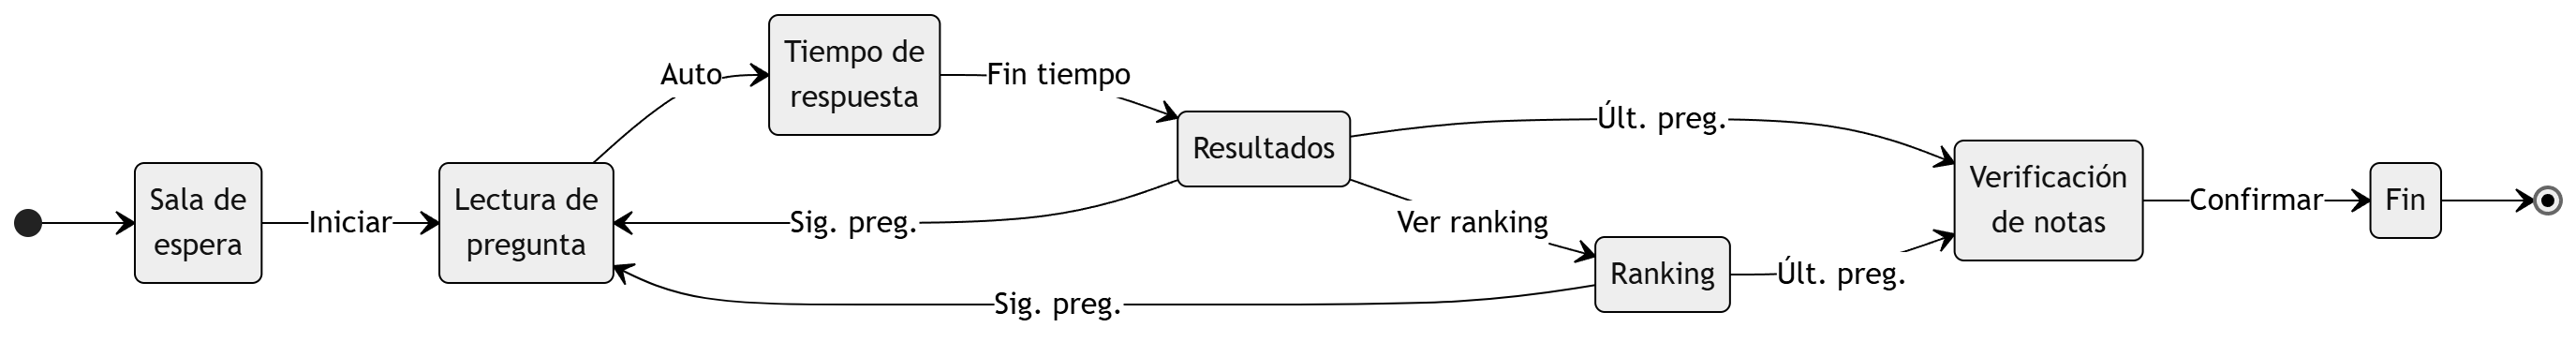
\includegraphics[width=1.2\textwidth]{figures/estados_sala.png}
    }
    \caption{Estados de la sala de juego en tiempo real.}
    \label{fig:estados_sala}
\end{figure}

El diseño de este comportamiento se apoya en los siguientes componentes conceptuales:
\begin{itemize}
    \item \textbf{Gestor centralizado de conexiones:} Mantiene el registro de las sesiones activas en memoria, administrando el ciclo de vida de los sockets y aplicando el patrón de difusión (\textit{broadcasting}) para emitir instrucciones a todos los participantes de una sala de forma simultánea.
    \item \textbf{Bucle de sincronización temporal:} Proceso asíncrono en segundo plano que supervisa el transcurso del tiempo de respuesta en las salas activas, notifica el tiempo restante periódicamente y desencadena automáticamente la transición de fase al expirar el tiempo.
    \item \textbf{Ciclo de eventos y transmisión:} Los cambios de estado de la sala (fase de lectura, apertura de respuestas, muestra de resultados, actualización de temporizadores) se propagan como eventos estructurados JSON, permitiendo que la interfaz del cliente reaccione de forma inmediata.
\end{itemize}

\begin{figure}[H]
    \centering
    \makebox[0pt][c]{
        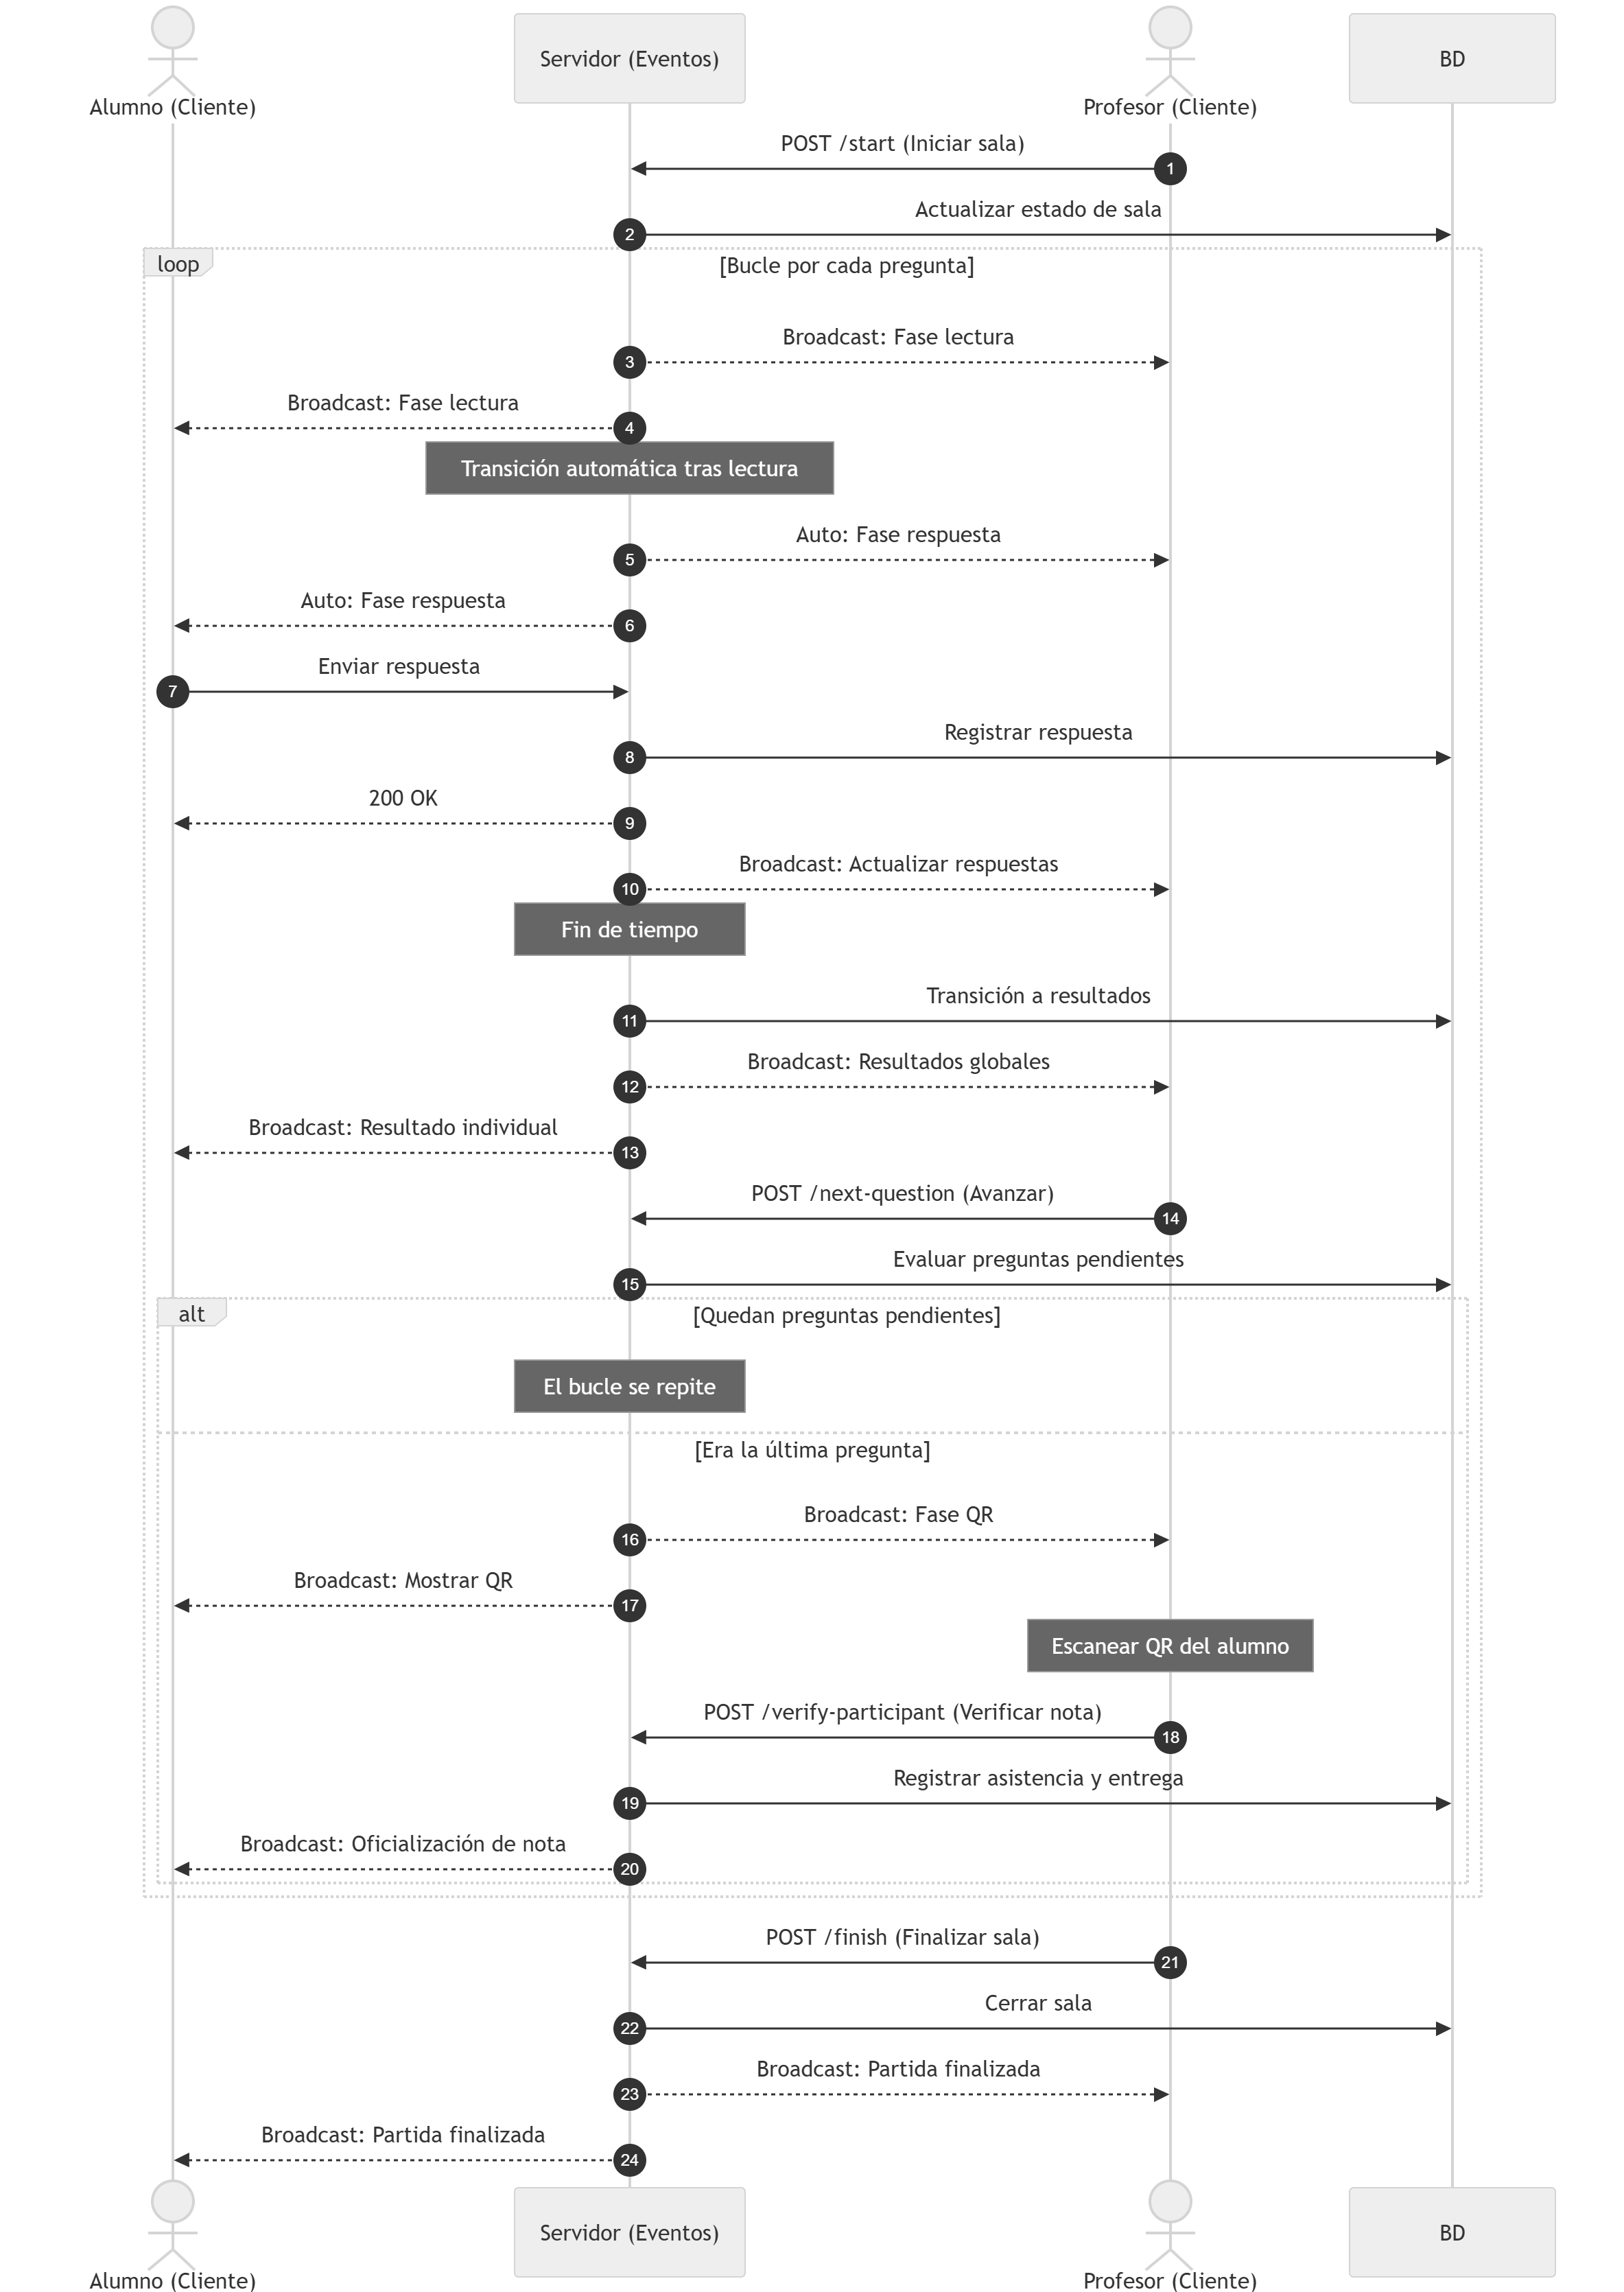
\includegraphics[width=1.06\textwidth]{figures/diagrama_secuencia_eventos.png}
    }
    \caption{Diagrama de secuencia de la transmisión de eventos en una sala.}
    \label{fig:diagrama_secuencia_eventos}
\end{figure}

\section{Arquitectura global del sistema}

La combinación de los tres patrones previamente descritos se consolida en una estructura global unificada. Como se ilustra en el \hyperref[fig:arquitectura_global]{esquema de la arquitectura global} del sistema, este enfoque permite integrar en un único marco de trabajo los terminales cliente, los canales de comunicación síncronos y asíncronos, las capas de servicios del \textit{backend} y el sistema de persistencia de datos.

\begin{figure}[H]
    \centering
    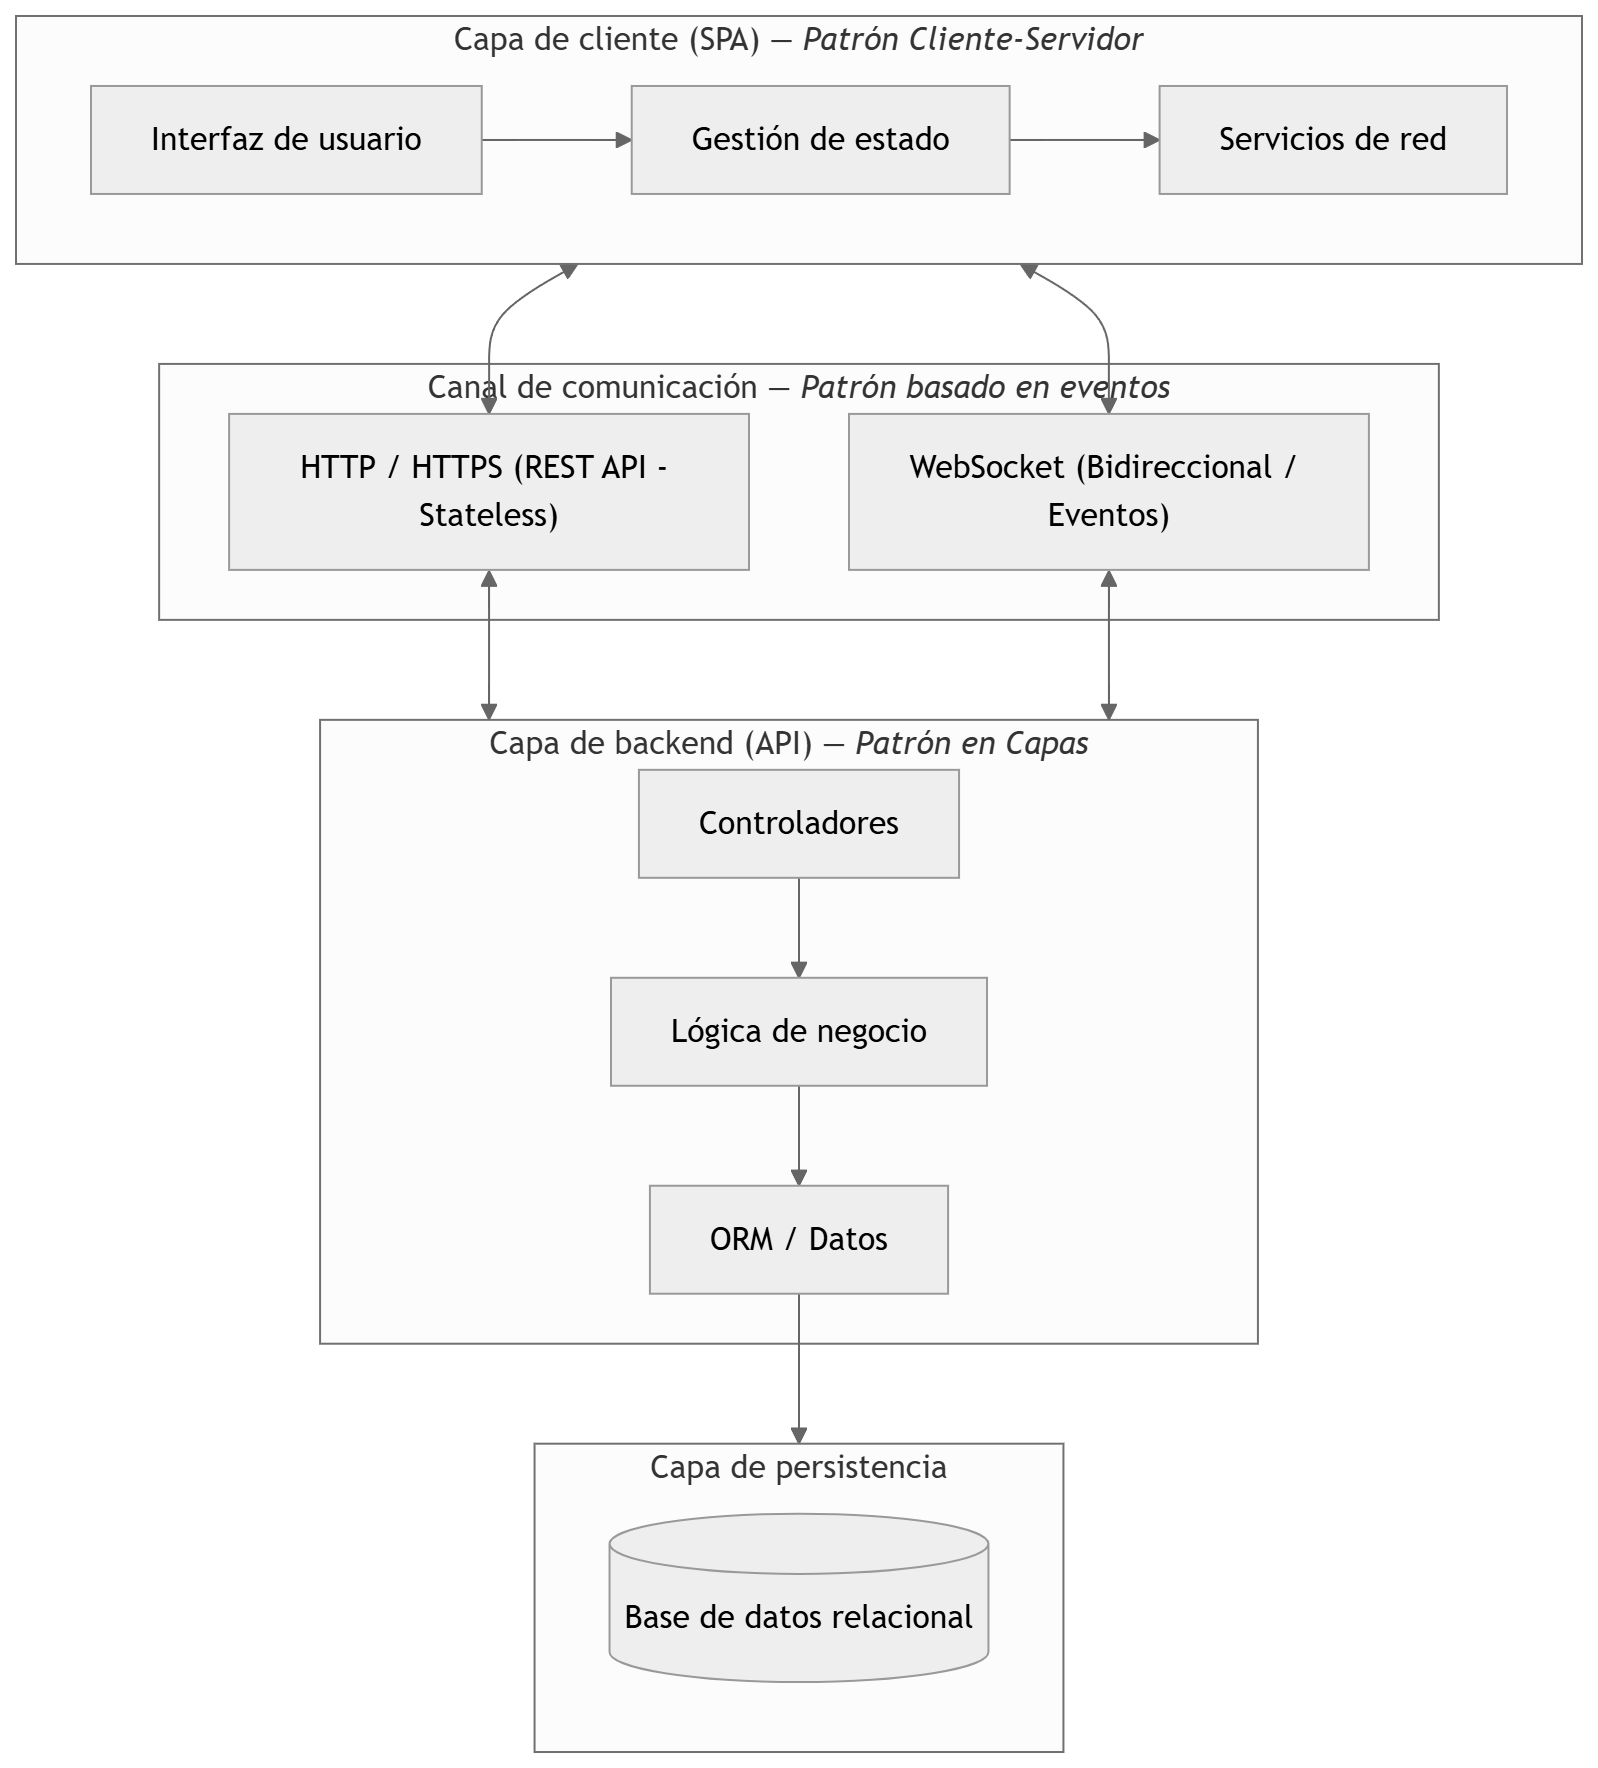
\includegraphics[width=0.85\textwidth]{figures/arquitectura_global.png}
    \caption{Esquema de la arquitectura global del sistema.}
    \label{fig:arquitectura_global}
\end{figure}

\section{Estructura modular del código}
Organización del proyecto en módulos independientes tanto para el Frontend (React) como para el Backend (FastAPI), facilitando la escalabilidad y el mantenimiento

Hablar de la organización del código en módulos independientes, explicando cómo se han estructurado y por qué es importante para la escalabilidad y el mantenimiento del proyecto.

\section{Modelo de datos}
Diagrama de dominio

Incluir el código mermaid y el diagrama

\section{Diseño de interfaces}
Mockups y resultado final

Mostrar los mockups iniciales y compararlos con el resultado final, explicando las decisiones de diseño tomadas y cómo se han implementado en la interfaz de usuario.

\section{Seguridad}
Autenticación JWT,  gestión de roles y tokens de verificación para participantes

\section{Documentación de la API}
Descripción de los endpoints principales de la API, detallando las peticiones, respuestas y la integración con el estándar OpenAPI

Aquí exprimiría el Swagger
